\documentclass[12pt]{report}
\usepackage[utf8]{inputenc}
\usepackage[russian]{babel}
%\usepackage[14pt]{extsizes}
\usepackage{listings}

% Для листинга кода:
\lstset{ %
language=python,                 % выбор языка для подсветки (здесь это С)
basicstyle=\small\sffamily, % размер и начертание шрифта для подсветки кода
numbers=left,               % где поставить нумерацию строк (слева\справа)
numberstyle=\tiny,           % размер шрифта для номеров строк
stepnumber=1,                   % размер шага между двумя номерами строк
numbersep=5pt,                % как далеко отстоят номера строк от подсвечиваемого кода
showspaces=false,            % показывать или нет пробелы специальными отступами
showstringspaces=false,      % показывать или нет пробелы в строках
showtabs=false,             % показывать или нет табуляцию в строках
frame=single,              % рисовать рамку вокруг кода
tabsize=2,                 % размер табуляции по умолчанию равен 2 пробелам
captionpos=t,              % позиция заголовка вверху [t] или внизу [b] 
breaklines=true,           % автоматически переносить строки (да\нет)
breakatwhitespace=false, % переносить строки только если есть пробел
escapeinside={\#*}{*)}   % если нужно добавить комментарии в коде
}

% Для измененных титулов глав:
\usepackage{titlesec, blindtext, color} % подключаем нужные пакеты
\definecolor{gray75}{gray}{0.75} % определяем цвет
\newcommand{\hsp}{\hspace{20pt}} % длина линии в 20pt
% titleformat определяет стиль
\titleformat{\chapter}[hang]{\Huge\bfseries}{\thechapter\hsp\textcolor{gray75}{|}\hsp}{0pt}{\Huge\bfseries}


% plot
\usepackage{pgfplots}
\usepackage{filecontents}
\usetikzlibrary{datavisualization}
\usetikzlibrary{datavisualization.formats.functions}

\begin{document}
 
%\def\chaptername{} % убирает "Глава"
\begin{titlepage}
	\centering
	{\scshape\LARGE МГТУ им. Баумана \par}
	\vspace{3cm}
	{\scshape\Large Лабораторная работа №6\par}
	\vspace{0.5cm}	
	{\scshape\Large По курсу: "Анализ алгоритмов"\par}
	\vspace{1.5cm}
	{\huge\bfseries Муравьиный алгоритм\par}
	\vspace{2cm}
	\Large Работу выполнил: студент группы ИУ7-53Б Наместник Анастасия\par
	\vspace{0.5cm}
	\LargeПреподаватели:  Волкова Л.Л., Строганов Ю.В.\par

	\vfill
	\large \textit {Москва, 2020} \par
\end{titlepage}

\tableofcontents

\newpage
\chapter*{Введение}
\addcontentsline{toc}{chapter}{Введение}

	\textbf{Муравьиный алгоритм}(алгоритм оптимизации подражанием муравьиной колонии) — один из эффективных полиномиальных алгоритмов для нахождения приближённых решений задачи коммивояжёра, а также решения аналогичных задач поиска маршрутов на графах\cite{OLNA}. 
	
Иными словами, это -  семейство приближенных алгоритмов для решения различных сложных оптимизационных задач. Идея этих алгоритмов основана на моделировании поведения муравьиной колонии, выполняющей поиск пути от муравеййника к источнику пищи. Первый вариант муравьиного алгоритма, предназначенный для приближенного решения задачи коммивояжера, был разработан Марко Дориго в 1992 году\cite{Lecture}.

Муравьиные алгоритмы серьезно исследуются европейскими учеными с середины 1990-х годов. Уже получены хорошие результаты муравьиной оптимизации для многих сложных комбинаторных задач: задачи коммивояжера, оптимизации маршрутов грузовиков, раскраски графа, квадратичной задачи о назначениях, оптимизации сетевых графиков, задачи календарного планирования и других. Особенно эффективны муравьиные алгоритмы при on-line оптимизации процессов в распределенных нестационарных системах, например трафиков в телекоммуникационных сетях\cite{AntAlg}.

Целью данной лабораторной работы является изучение муравьиных алгоритмов и приобретение навыков параметризации методов на примере муравьиного алгоритма, примененного к задаче коммивояжера.

В данной лабораторной работе требуется решить пять задач:
\begin{itemize}
\item изучить алгоритм полного перебора для решения задачи коммивояжера;
\item изучить муравьиный алгоритм для решения задачи коммивояжера;
\item программно реализовать описанные выше алгоритмы;
\item провести параметризацию муравьиного алгоритма на классе данных;
\item провести сравнительный анализ скорости работы реализованных алгоритмов.
\end{itemize}


\chapter{Аналитическая часть}

В этом разделе будут представлены теоретические сведения, необходимые для программной реализации муравьиного алгоритма, примененного к задаче коммивояжера.
 
\section{Понятие коммивояжера}
 Коммивояжёр (фр. commis voyageur) — бродячий торговец. Задача коммивояжёра — важная задача транспортной логистики, отрасли, занимающейся планированием транспортных перевозок. Коммивояжёру, чтобы распродать нужные и не очень нужные в хозяйстве товары, следует объехать n пунктов и в конце концов вернуться в исходный пункт. Требуется определить наиболее выгодный маршрут объезда. В качестве меры выгодности маршрута (точнее говоря, невыгодности) может служить суммарное время в пути, суммарная стоимость дороги, или, в простейшем случае, длина маршрута\cite{Commis}.

\section{Решение полным перебором}
Совершенно очевидно, что задача может быть решена перебором всех вариантов объезда и выбором оптимального. Но при таком подходе количество возможных маршрутов очень быстро возрастает с ростом n (оно равно n! — количеству способов упорядочения пунктов). К примеру, для 100 пунктов количество вариантов будет представляться 158-значным числом. Мощная ЭВМ, способная перебирать миллион вариантов в секунду, будет решать такую задачу на протяжении примерно 3*10144 лет. Увеличение производительности ЭВМ в 1000 раз даст хоть и меньшее в 1000 раз, но по-прежнему очень большое время перебора вариантов. Не спасает ситуацию даже то, что для каждого варианта маршрута имеется 2n равноценных, отличающихся выбором начального пункта (n вариантов) и направлением обхода (2 варианта). Перебор с учётом этого наблюдения сокращается незначительно. 

Таким образом, хотя такой подход и гарантирует точное решение задачи, уже при небольшом числе городов решение за допустимое количество времени невозможно.\cite{Brute}. 	

\section{Решение с помощью муравьиного алгоритма}
В то время как простой метод перебора всех вариантов чрезвычайно неэффективный при большом количестве городов, эффективными признаются решения, гарантирующие получение ответа за время, ограниченное полиномом от размерности задачи. С помощью муравьиных алгоритмов находятся субоптимальные решения, локальные минимумы целевой функции, приближающиеся к абсолютному минимуму\cite{AntAlg}.

В основе алгоритма лежит поведение муравьиной колонии — маркировка более удачных путей большим количеством феромона. Рассмотрим биологическую модель поведения такой колонии.

В реальном мире муравьи (первоначально) ходят в случайном порядке и по нахождении продовольствия возвращаются в свою колонию, прокладывая феромонами тропы. Если другие муравьи находят такие тропы, они, вероятнее всего, пойдут по ним. Вместо того, чтобы отслеживать цепочку, они укрепляют её при возвращении, если в конечном итоге находят источник питания. Со временем феромонная тропа начинает испаряться, тем самым уменьшая свою привлекательную силу. Чем больше времени требуется для прохождения пути до цели и обратно, тем сильнее испарится феромонная тропа. На коротком пути, для сравнения, прохождение будет более быстрым, и, как следствие, плотность феромонов остаётся высокой. Испарение феромонов также имеет функцию избежания стремления к локально-оптимальному решению. Если бы феромоны не испарялись, то путь, выбранный первым, был бы самым привлекательным. В этом случае, исследования пространственных решений были бы ограниченными. Таким образом, когда один муравей находит (например, короткий) путь от колонии до источника пищи, другие муравьи, скорее всего пойдут по этому пути, и положительные отзывы в конечном итоге приводят всех муравьёв к одному, кратчайшему, пути. Этапы работы муравьиной колонии представлены на рис. 2.1.

\begin{center}
		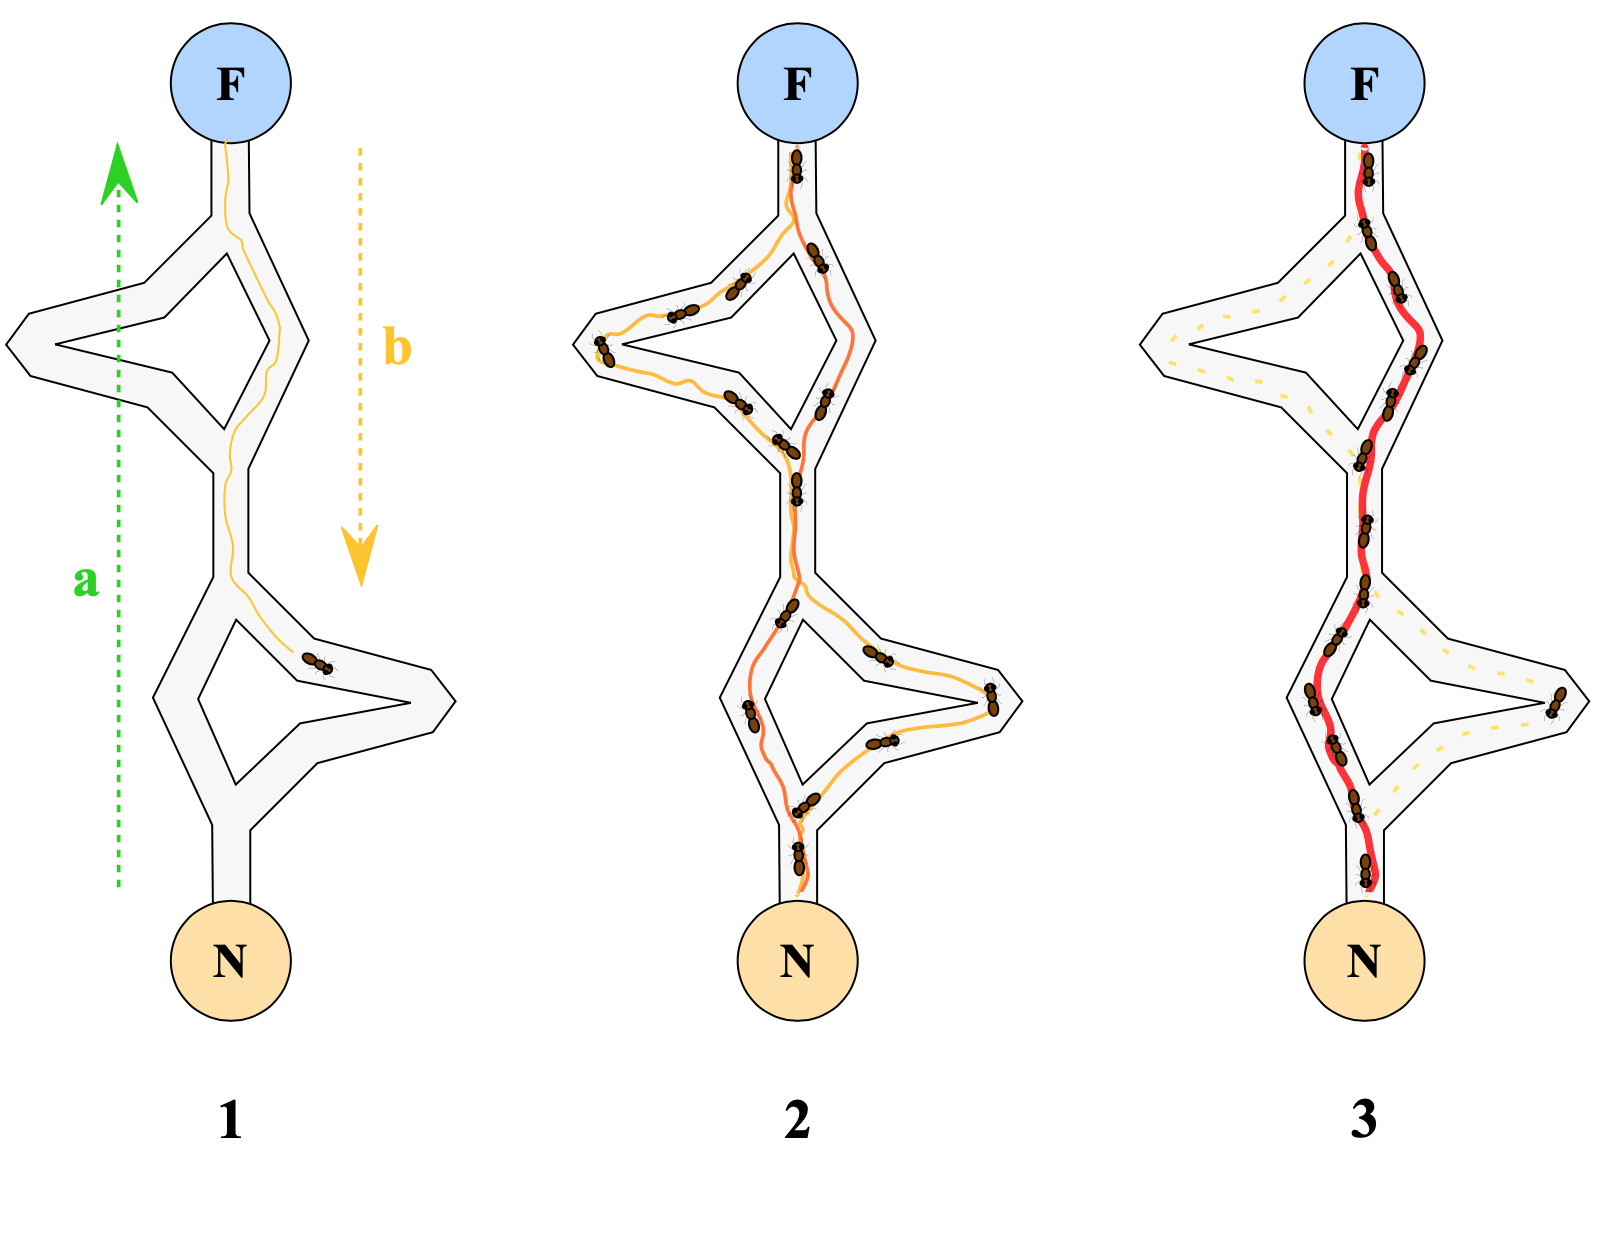
\includegraphics[scale=0.4]{pics/Ants.png}
		
			Рис 2.1: Работа муравьиной колонии
\end{center}

Оригинальная идея исходит от наблюдения за муравьями в процессе поиска кратчайшего пути от колонии до источника питания.
\begin{enumerate}
\item Первый муравей находит источник пищи (F) любым способом (а), а затем возвращается к гнезду (N), оставив за собой тропу из феромонов (b).
\item Затем муравьи выбирают один из четырёх возможных путей, затем укрепляют его и делают привлекательным.
\item программно реализовать описанные выше алгоритмы;
\item Муравьи выбирают кратчайший маршрут, так как феромоны с более длинных путей быстрее испаряются.
\end{enumerate}

Теперь рассмотрим каждый шаг в цикле более подробно:\\

1. Создание муравьев\\
   Стартовая точка, куда помещается муравей, зависит ограничений,   накладываемых условиями задачи. Потому что для каждой задачи   способ размещения муравьёв является определяющим. Либо все они помещаются в одну точку, либо в разные с повторения, либо без повторений. \\
  На этом же этапе задается начальный уровень феромона. Он инициализируется небольшим положительным числом для того, чтобы на начальном шаге вероятности перехода в следующую  вершину не были нулевыми. \\
  
2. Поиск решения  \\
 Вероятность перехода из вершины i в вершину j определяется по следующей формуле\ref{form:way}\\   
\begin{equation}\label{form:way} 
 p_{i,j}={\frac {(\tau_{i,j}^{\alpha })(\eta_{i,j}^{\beta })}{\sum (\tau_{i,j}^{\alpha })(\eta_{i,j}^{\beta })}}
 \end{equation}
    где \quad$ \tau_{i,j} - $ расстояние от города i до j;
    
         $\eta_{i,j} - $количество феромонов на ребре ij;
         
          $\alpha - $ параметр влияния длины пути;
          
          $\beta - $ параметр влияния феромона.


3. Обновление феромона \\
  Уровень феромона обновляется в соответствии с приведённой формулой:\\
После того, как муравей успешно проходит маршрут, он оставляет на всех пройденных ребрах след, обратно пропорциональный длине пройденного пути. Итого, новый след феромона вычисляется по формуле \ref{form:eva}:
\begin{equation}\label{form:eva} 
    \tau_{i,j}=(1-\rho )\tau_{i,j}+\Delta \tau_{i,j},
\end{equation}

где \quad$ \rho_{i,j}$ - \text{доля феромона, который испарится;} 

    $\tau_{i,j}$ - \text{количество феромона на дуге ij;} 
    
    $\Delta \tau_{i,j}$ - \text{количество отложенного феромона, вычисляется по формуле \ref{form:add1}.}


\section{Формализация задачи коммивояжера в терминах подхода муравьиных алгоритмов}
Рассмотрим, как реализовать четыре составляющие самоорганизации муравьев при оптимизации маршрута коммивояжера. Многократность взаимодействия реализуется итерационным поиском маршрута коммивояжера одновременно несколькими муравьями. При этом каждый муравей рассматривается как отдельный, независимый коммивояжер, решающий свою задачу. За одну итерацию алгоритма каждый муравей совершает полный маршрут коммивояжера.Положительная обратная связь реализуется как имитация поведения муравьев типа «оставление следов – перемещение по следам». Чем больше следов оставлено на тропе — ребре графа в задаче коммивояжера, тем больше муравьев будет передвигаться по ней. При этом на тропе появляются новые следы, привлекающие дополнительных муравьев. Для задачи коммивояжера положительная обратная связь реализуется следующим стохастическим правилом: вероятность включения ребра графа в маршрут муравья пропорциональна количеству феромона на нем.
		
Теперь с учетом особенностей задачи коммивояжёра, можно описать локальные правила поведения муравьев при выборе пути.
		
	1. Муравьи имеют собственную «память». Поскольку каждый город может быть посещён только один раз, то у каждого муравья есть список уже посещенных городов - список запретов. Обозначим через $J$ список городов, которые необходимо посетить муравью $k$ , находящемуся в городе $i$ . 
	
	2. Муравьи обладают «зрением» - видимость есть эвристическое желание посетить город $j$ , если муравей находится в городе $i$ . Будем считать, что видимость обратно пропорциональна расстоянию между городами. 
	
	3. Муравьи обладают «обонянием» - они могут улавливать след феромона, подтверждающий желание посетить город $j$ из города $i$ на основании опыта других муравьёв. Количество феромона на ребре $(i,j)$ в момент времени $t$ обозначим через  $tau_{i,j} (t)$ 
	
	 4. На этом основании мы можем сформулировать вероятностно-пропорциональное правило, определяющее вероятность перехода $k$-ого муравья из города $i$  в город $j$. 
	 
	5. Пройдя ребро $(i,j)$ , муравей откладывает на нём некоторое количество феромона, которое должно быть связано с оптимальностью сделанного выбора. Пусть $T _{k} (t)$ есть маршрут, пройденный муравьем $k$ к моменту времени $t$ , $L _{k} (t)$ - длина этого маршрута, а $Q$ - параметр, имеющий значение порядка длины оптимального пути. Тогда откладываемое количество феромона может быть задано в виде:
	
 \begin{equation}\label{form:add} 
    {\displaystyle \Delta \tau_{i,j}^k={\begin{cases}Q/L_{k}& {\mbox{Если k-ый мурваей прошел по ребру ij;}}\\0&{\mbox{Иначе}}\end{cases}}}
\end{equation}
   где \quad Q - количество феромона, переносимого муравьем;
   
 Тогда
 \begin{equation}\label{form:add1} 
    \Delta \tau_{i,j}= \tau_{i,j}^0 + \tau_{i,j}^1 + ... + \tau_{i,j}^k 
\end{equation}
   
    где k - количество муравьев в вершине графа с индексами i и j.



\section{Вывод}

В данном разделе были рассмотрены теоретические сведения, необходимые для программной реализации муравьиного алгоритма, примененного к задаче коммивояжера..
 
\chapter{Конструкторская часть}

В данном разделе будут представлены схемы реализации алгоритма полного перебора и муравьиного алгоритма для решения задачи коммивояжера.

Схема реализации алгоритма полного перебора представлена на рис. 2.2.

\begin{center}
		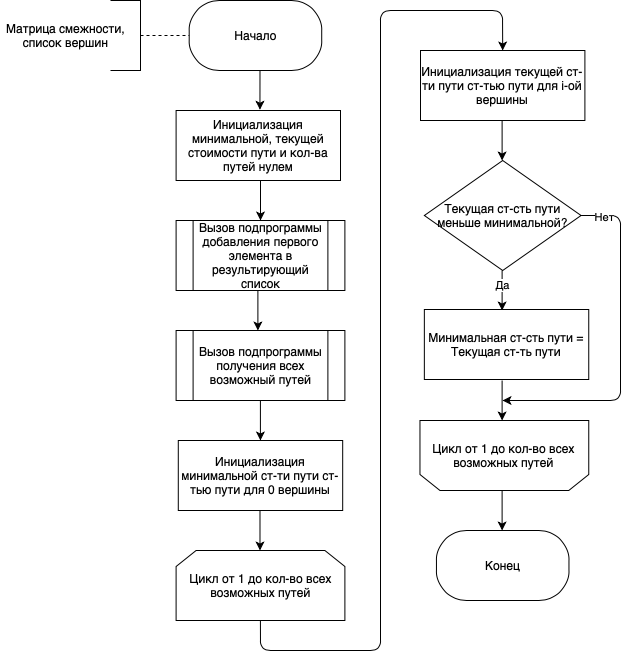
\includegraphics[scale=0.6]{schema/Brute.png}
		
			Рис 2.2: Схема реализации алгоритма полного перебора
\end{center}

Схема реализации муравьиного алгоритма представлена на рис. 2.3.

\begin{center}
		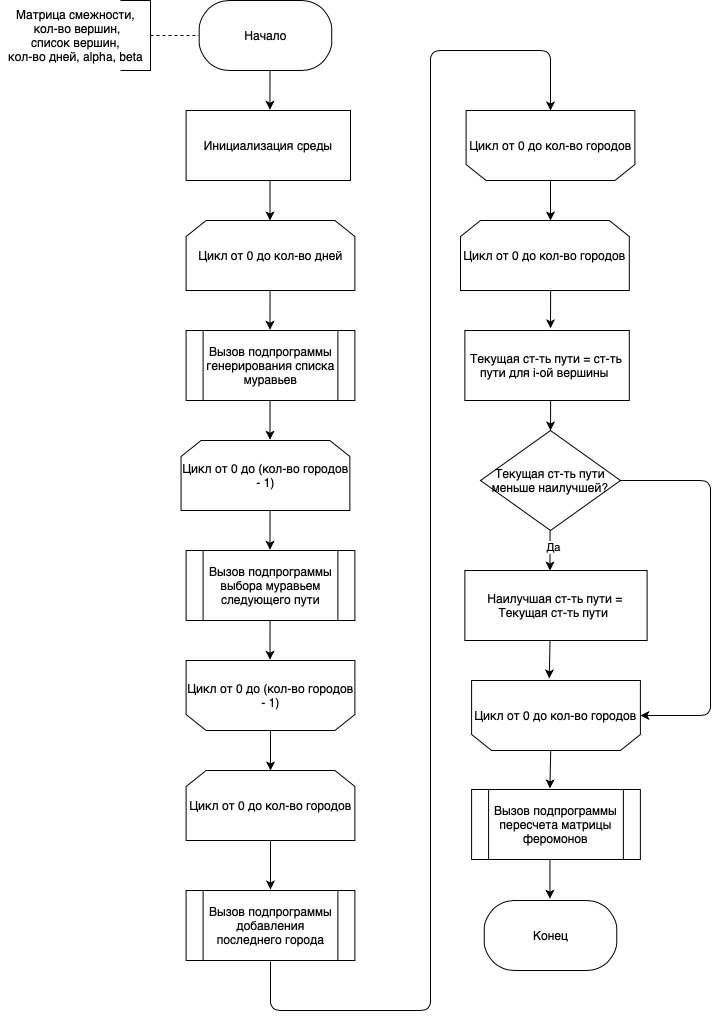
\includegraphics[scale=0.6]{schema/Ants.png}
		
			Рис 2.3: Схема реализации муравьиного алгоритма 
\end{center}


\section{Вывод}
В данном разделе были рассмотрены 2 схемы: схема программной реализации алгоритма полного перебора и схема программной реализации муравьиного алгоритма. 

\chapter{Технологическая часть}
\section{Выбор языка программирования}
В данной лабораторной работе использовался язык программирования - С \cite{C}, так как данный язык программирования предоставляет удобные библиотеки и инструменты для работы со структурами данных и обеспечивает хорошую производительность программного продукта. В качестве интегрированной среды разработки использовалась Visual studio  \cite{Vs}.  

\section{Сведения о модулях программы}
Программа состоит из следующих модулей:
\begin{itemize}
	\item main.c - главный файл программы, в котором располагается точка входа в программу;
	\item ant\_algorithm.c - реализация муравьиного алгоритма;
	\item brute\_force.c - реализация алгоритма полного перебора;
	\item matrix.c - модуль для работы с матрицей смежности;
	\item array.c - модуль для организации списка;
	\item city.c - модуль для организации списка городов;
	\item parser.c - модуль для представления результата в графическом виде.
\end{itemize}

На листинге 3.1 представлена подпрограмма точки входа main().
\begin{lstlisting}[label=some-code,caption= Код подпрограммы main()]

int main(int argc, char *argv[])
{
    srand(time(NULL));

    array cities; 

    char city_names[LEN]; 
    int matrix[LEN][LEN]; 

    FILE *f = fopen(argv[1], "r");

    if (!f)
    {
        printf("Error.\n");
        return ERROR_OPEN_FILE;
    }

    int count = parser(f, city_names, matrix);

    fclose(f);

    create_cities_array(&cities, count);

    print_cities(cities, city_names);
    print_matrix(matrix, count);

    array result = get_shortest_path(cities, matrix);
    int min_path_simple = get_path_cost(result, matrix);
    print_array(result, "result");
    red();
    printf("result simple = %d\n", min_path_simple);

    array result_ant = ant_algorithm(matrix, count, cities, 40, 0.4, 0.7, 0.3);
    int min_path_ant = get_path_cost(result_ant, matrix);
    print_array(result_ant, "result ant");
    red();
    printf("result ant = %d\n", min_path_ant);

    return OK;
}
\end{lstlisting}

На листинге 3.2 представлена реализация муравьиного алгоритма.

\begin{lstlisting}[label=some-code,caption=Реализация муравьиного алгоритма]
int calculate_Q(int matrix[LEN][LEN], int count)
{
	int Q = 0;

	for (int i = 0; i < count; i++)
		for (int j = 0; j < i; j++)
			Q += matrix[i][j];

	return Q * 2;
}

void add_pheromones(int matrix[LEN][LEN], float matrix_pheromones[LEN][LEN], int count, int Q, ant ants[ANTS_MAX_COUNT])
{
	int city_first, city_second;
	int curr_cost;
	float delta_tao = 0;
	
	for (int i = 0; i < count; i++)
	{
		curr_cost = get_path_cost(ants[i].way, matrix);

		delta_tao += (float)Q / curr_cost;

		// printf("Q = %d; curr_cost = %d; delta_tao = %f\n", Q, curr_cost, delta_tao);
	}

		for (int i = 0; i < count; i++)
	{
		for (int j = 0; j < ants[i].way.count - 1; j++)
		{
			city_first = ants[i].way.arr[j];
			city_second = ants[i].way.arr[j + 1];
		
			matrix_pheromones[city_first][city_second] = matrix_pheromones[city_first][city_second] + delta_tao;
			matrix_pheromones[city_second][city_first] = matrix_pheromones[city_second][city_first] + delta_tao;
		}
		// printf("\n");
	}
}

void correct_pheromones(float matrix_pheromones[LEN][LEN], int count)
{
	for (int i = 0; i < count; i++)
		for (int j = 0; j < i; j++)
			if (matrix_pheromones[i][j] <= 0.1)
				matrix_pheromones[i][j] = matrix\_pheromones[j][i] = 0.1;
}

void evaporation(float matrix_pheromones[LEN][LEN], int count, float p)
{
	float tmp = 1 - p;
	for (int i = 0; i < count; i++)
		for (int j = 0; j < i; j++)
		{
			matrix_pheromones[i][j] = tmp * matrix_pheromones[i][j];
			matrix_pheromones[j][i] = tmp * matrix_pheromones[j][i];
		}
}

void print_matrix_pheromones(float matrix_pheromones[LEN][LEN], int count)
{
	for (int i = 0; i < count; i++)
	{
		for (int j = 0; j < count; j++)
			printf("%f ", matrix_pheromones[i][j]);
		printf("\n");
	}
}

array ant_algorithm(int matrix[LEN][LEN], int count, array cities, int tmax, float p, float alpha, float beta)
{
	int Q = calculate_Q(matrix, count);

	array best_way = copy_arr(cities);
	add_elem(&best_way, get_elem(best_way, 0));
	
	int best_cost = get_path_cost(best_way, matrix);
	int curr_cost = 0;
	
	float matrix_pheromones[LEN][LEN];
	fill_matrix(matrix_pheromones, count, PHEROMONE\_MIN);

	ant ants[ANTS_MAX_COUNT];

	for (int t = 0; t < tmax; t++)
	{
		generate_ants_array(ants, count);

		for (int i = 0; i < count - 1; i++)
		{
			ants_choose_way(ants, matrix_pheromones, matrix, count, alpha, beta);
		}

		for (int i = 0; i < count; i++)
			add_elem(&ants[i].way, get_elem(ants[i].way, 0));

		for (int i = 0; i < count; i++)
		{
			curr_cost = get_path_cost(ants[i].way, matrix);
			if (curr_cost < best_cost)
			{
				best_cost = curr_cost;
				best_way = copy_arr(ants[i].way);
			}
		}

		evaporation(matrix_pheromones, count, p);
		add_pheromones(matrix, matrix_pheromones, count, Q, ants);
		correct_pheromones(matrix_pheromones, count);
	}

	return best_way;
}

\end{lstlisting}

На листинге 3.3 представлена реализация алгоритма полного перебора.

\begin{lstlisting}[label=some-code,caption=Реализация алгоритма полного перебора]
int get_path_cost(array cities, int matrix[LEN][LEN])
{
	int cost = 0;

	for (int i = 0; i < cities.count - 1; i++)
		cost += matrix[cities.arr[i]][cities.arr[i + 1]];

	return cost;
}

array get_shortest_path(array cities, int matrix[LEN][LEN])
{
	array result[DEPTH_OF_RECURSION];
	array res_arr;

	int min_cost;
	int curr_cost;
	int index = 0;

	int routes_count = 0;

	del_elem(&cities, 0);
	add_elem(&res_arr, 0);
	get_routes(&cities, &res_arr, result, &routes_count);

	min_cost = get_path_cost(result[index], matrix);
	
	for (int i = 1; i < routes_count; i++)
	{
		curr_cost = get_path_cost(result[i], matrix);
		
		if (curr_cost < min_cost)
		{
			min_cost = curr_cost;
			index = i;
		}
	}

	return result[index];
}

void get_routes(array *cities, array *res_arr, array result[DEPTH_OF_RECURSION], int *count)
{
	int elem;
	array tmp;

	if (!cities->count)
	{
		add_elem(res_arr, get_elem(*res_arr, 0));
		result[*count] = *res_arr;
		(*count)++;
		del_elem(res_arr, res_arr->count - 1);
	}

	for (int i = 0; i < cities->count; i++)
	{
		elem = get_elem(*cities, i);
		
		add_elem(res_arr, elem);

		tmp = copy_arr(*cities);
		del_elem(&tmp, i);

		get_routes(&tmp, res_arr, result, count);

		del_elem(res_arr, res_arr->count - 1);
	}
}
\end{lstlisting}

На листинге 3.4 представлены подпрограммы инициализации и вывода матрицы смежности.

\begin{lstlisting}[label=some-code,caption=Подпрограммы инициализации и вывода матрицы смежности]
public static int FindMin(intPtr array)
void print_matrix(int matrix[LEN][LEN], int const count)
{
	blue();
	for (int i = 0; i < count; i++)
		printf("%d\t", i);
	puts("");

	for (int i = 0; i < count; i++)
	{
		printf("%d ", i);
		for (int j = 0; j < count; j++)
			printf("%d\t", matrix[i][j]);
		puts("");
	}
	puts("");
}

void fill_matrix(float matrix[LEN][LEN], int count, float num)
{
	for (int i = 0; i < count; i++)
		for (int j = 0; j < i; j++)
			matrix[i][j] = matrix[j][i] = num;
}
\end{lstlisting}

На листинге 3.5 представлены подпрограммы организации списка вершин (городов).

\begin{lstlisting}[label=some-code,caption=Подпрограммы организации списка вершин (городов)]
void print_array(array cities, char msg[MSG\_LEN])
{
	green();
	printf("%s\ncount: %d\n", msg, cities.count);
	yellow();
	for (int i = 0; i < cities.count; i++)
		printf("%d  ", cities.arr[i]);
	puts("\n");
	blue();
}

void add_elem(array *cities, const int elem)
{
	cities->arr[cities->count] = elem;
	(cities->count)++;
}

int get_elem(array array, int const index)
{
	if (index > array.count)
		return NOT_FOUND;

	return array.arr[index];
}

int del_elem(array *array, int const index)
{
	if (index > array->count)
		return NOT_FOUND;

	int tmp, elem = array->arr[index];

	for (int i = index; i < array->count; i++)
	{
		tmp = array->arr[i];
		array->arr[i] = array->arr[i + 1];
		array->arr[i + 1] = tmp;
	}

	(array->count)--;

	return elem;
}

array copy_arr(array arr)
{
	array result;
	result.count = arr.count;

	for (int i = 0; i < arr.count; i++)
		result.arr[i] = arr.arr[i];

	return result;
}\end{lstlisting}


\section{Вывод}
В технологической части были представлены модули программы, листинги кода, а также обусловлен выбор языка программирования и приведены использовавшиеся в ходе работы инструменты.

\chapter{Исследовательская часть}

В этом разделе будет проведен сравнительный анализ характеристик полученного программного продукта.

\section{Характеристики ЭВМ}

\begin{itemize}
	\item MacBook Pro (Retina, 15-inch, Mid 2014).
	\item 2,5 GHz Intel Core i7.
	\item Число логических ядер: 8.
\end{itemize}

\section{Временные характеристики} 

Результаты замеров времени приведены в таблице 4.1.

\begin{tabular}{|c c c|}
		\hline
		Размерность матрицы & Полный перебор & Муравьиный алгоритм  \\ [0.5ex] 
 		\hline\hline
		3 & 1612 & 89996\\
 		\hline
 		4 & 1441 & 151542\\
 		\hline
 		5 & 2319 & 286035\\
 		\hline
		6 & 7725 & 469782\\
		\hline
		7 & 43539 & 710305\\
		\hline
		8 & 305564 & 1039688\\
		\hline
		9 & 2500918 & 1470419\\
		\hline
		10 & 22690076 & 1886565\\
		\hline
\end{tabular}


На рис. 2.4 приведен графики зависимостей времени работы алгоритмов от размерности матрицы смежности.

\begin{center}
		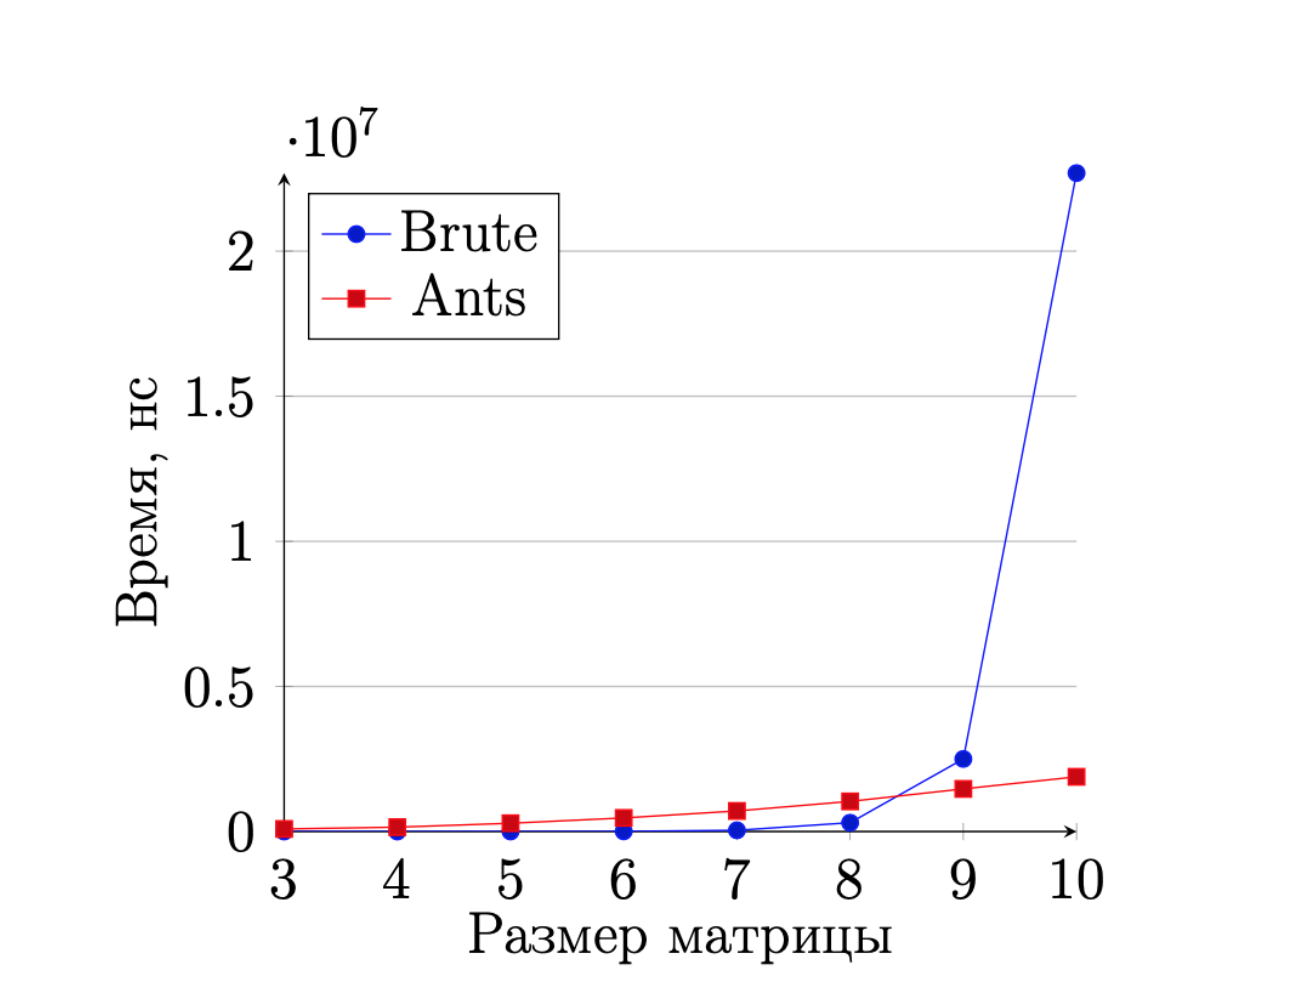
\includegraphics[scale=0.4]{pics/time.png}
		
			Рис 2.4: Зависимость времени работы алгоритмов от размерности матрицы смежности
\end{center}


В муравьином алгоритме вычисления производятся на основе настраиваемых параметров.
Рассмотрим два класса данных и подберем к ним параметры, при которых метод даст точный результат при небольшом количестве итераций.

Будем рассматривать матрицы размерности $10\times10$, так как иначе получение точного результата алгоритмом велико и менее зависимо от параметров.

В качестве первого класса данных выделим матрицу смежности, в которой все значения незначительно отличаются друг от друга, например, в диапазоне $[1, 25]$.
Вторым классом будут матрицы, где значения могут значительно отличаться, например $[1, 2500]$.

Будем запускать муравьиный алгоритм для всех значений $\alpha, \rho\in[0, 1]$, с шагом $= 0.1$, пока не будет найдено точное значение для каждого набора.

В результате тестирования будет выведена таблица со значениями $\alpha, \beta, \rho, Длина, Разница$, где Длина — оптимальная длина пути, найденная муравьиным алгоритмом, Разница - Разность между полученным значением и настоящей оптимальной длиной пути, а $\alpha, \beta, \rho$ — настраиваемые параметры.


\subsection{Класс данных}

\begin{tabular}{|c c c c c c c c c c|}
    \label{matrix}
  	 0 & 21 &  21 & 4 & 22 & 20 & 6 & 4 & 11 & 23 \\
        21 &     0 &    22 &     6 &     9 &    21 &    16 &     6 &     2 &     7 \\
        21 &    22 &     0 &    18 &    23 &     7 &    19 &    19 &     1 &    14 \\
        4 &     6 &    18 &     0 &     7 &    11 &    16 &    10 &     8 &    19 \\
        22 &     9 &    23 &     7 &     0 &    15 &     2 &    23 &     1 &    22 \\
        20 &    21 &     7 &    11 &    15 &     0 &     6 &     7 &     8 &    21 \\
        6 &    16 &    19 &    16 &     2 &     6 &     0 &     8 &     3 &    14 \\
        4 &     6 &    19 &    10 &    23 &     7 &     8 &     0 &    23 &    15 \\
        11 &     2 &     1 &     8 &     1 &     8 &     3 &    23 &     0 &     9 \\
        23 &     7 &    14 &    19 &    22 &    21 &    14 &    15 &     9 &     0 \\
 \end{tabular}

В таблице ~\ref{tab:log1} приведены результаты параметризации метода решения задачи коммивояжера на основании муравьиного алгоритма. Количество дней было взято равным 50. Полный перебор определил оптимальную длину пути 52. Два последних стобца таблицы определяют найденный муравьиным алгоритм оптимальный путь и разницу этого пути с оптимальным путём, найденным алгоритмом полного перебора.

\begin{table}
    \caption{Таблица коэффициентов для класса данных 1.}
    \begin{minipage}[h!]{0.10\hsize}\centering
        \begin{center}\resizebox{4\textwidth}{!}{%
                \begin{tabular}{|c@{\hspace{5mm}}|c@{\hspace{5mm}}|c@{\hspace{5mm}}|c@{\hspace{5mm}}|c@{\hspace{5mm}}|c|}
                    \hline
                    \alpha        & \beta      & \rho      &Длина  & Разница \\
                    \hline
                    0    & 1    & 0    & 52    & 0     \\
                    0    & 1    & 0.1  & 52    & 0     \\
                    0    & 1    & 0.2  & 52    & 0     \\
                    0    & 1    & 0.3  & 52    & 0     \\
                    0    & 1    & 0.4  & 53    & 1     \\
                    0    & 1    & 0.5  & 52    & 0     \\
                    0    & 1    & 0.6  & 52    & 0     \\
                    0    & 1    & 0.7  & 52    & 0     \\
                    0    & 1    & 0.8  & 52    & 0     \\
                    0    & 1    & 0.9  & 52    & 0     \\
                    0    & 1    & 1    & 52    & 0     \\
                    0.1  & 0.9  & 0    & 52    & 0     \\
                    0.1  & 0.9  & 0.1  & 52    & 0     \\
                    0.1  & 0.9  & 0.2  & 53    & 1     \\
                    0.1  & 0.9  & 0.3  & 52    & 0     \\
                    0.1  & 0.9  & 0.4  & 52    & 0     \\
                    0.1  & 0.9  & 0.5  & 52    & 0     \\
                    0.1  & 0.9  & 0.6  & 53    & 1     \\
                    0.1  & 0.9  & 0.7  & 52    & 0     \\
                    0.1  & 0.9  & 0.8  & 52    & 0     \\
                    0.1  & 0.9  & 0.9  & 52    & 0     \\
                    0.1  & 0.9  & 1    & 52    & 0     \\
                    0.2  & 0.8  & 0    & 52    & 0     \\
                    0.2  & 0.8  & 0.1  & 52    & 0     \\
                    0.2  & 0.8  & 0.2  & 52    & 0     \\
                    0.2  & 0.8  & 0.3  & 53    & 1     \\
                    0.2  & 0.8  & 0.4  & 52    & 0     \\
                    0.2  & 0.8  & 0.5  & 52    & 0     \\
                    0.2  & 0.8  & 0.6  & 53    & 1     \\
                    0.2  & 0.8  & 0.7  & 53    & 1     \\
                    0.2  & 0.8  & 0.8  & 52    & 0     \\
                    0.2  & 0.8  & 0.9  & 52    & 0     \\
                    0.2  & 0.8  & 1    & 52    & 0     \\
                    0.3  & 0.7  & 0    & 53    & 1     \\
                    0.3  & 0.7  & 0.1  & 52    & 0     \\
                    0.3  & 0.7  & 0.2  & 52    & 0     \\
                    0.3  & 0.7  & 0.3  & 53    & 1     \\
                    0.3  & 0.7  & 0.4  & 52    & 0     \\
                    0.3  & 0.7  & 0.5  & 52    & 0     \\
                    0.3  & 0.7  & 0.6  & 52    & 0     \\
                \end{tabular}}
                \label{tab:log1}
        \end{center}
    \end{minipage}
    \hfill
    \begin{minipage}[!h]{0.50\hsize}\centering
        \begin{center}\resizebox{0.8\textwidth}{!}{%
                %\caption{Лог работы программы.}
                \begin{tabular}{|c@{\hspace{5mm}}|c@{\hspace{5mm}}|c@{\hspace{5mm}}|c@{\hspace{5mm}}|c@{\hspace{5mm}}|c|}
                    \alpha        & \beta      & \rho      &Длина  & Разница \\
                    \hline
                    0.3  & 0.7  & 0.7  & 52    & 0     \\
                    0.3  & 0.7  & 0.8  & 52    & 0     \\
                    0.3  & 0.7  & 0.9  & 53    & 1     \\
                    0.3  & 0.7  & 1    & 52    & 0     \\
                    0.4  & 0.6  & 0    & 53    & 1     \\
                    0.4  & 0.6  & 0.1  & 53    & 1     \\
                    0.4  & 0.6  & 0.2  & 53    & 1     \\
                    0.4  & 0.6  & 0.3  & 52    & 0     \\
                    0.4  & 0.6  & 0.4  & 53    & 1     \\
                    0.4  & 0.6  & 0.5  & 52    & 0     \\
                    0.4  & 0.6  & 0.6  & 52    & 0     \\
                    0.4  & 0.6  & 0.7  & 52    & 0     \\
                    0.4  & 0.6  & 0.8  & 52    & 0     \\
                    0.4  & 0.6  & 0.9  & 52    & 0     \\
                    0.4  & 0.6  & 1    & 52    & 0     \\
                    0.5  & 0.5  & 0    & 52    & 0     \\
                    0.5  & 0.5  & 0.1  & 52    & 0     \\
                    0.5  & 0.5  & 0.2  & 52    & 0     \\
                    0.5  & 0.5  & 0.3  & 53    & 1     \\
                    0.5  & 0.5  & 0.4  & 52    & 0     \\
                    0.5  & 0.5  & 0.5  & 52    & 0     \\
                    0.5  & 0.5  & 0.6  & 52    & 0     \\
                    0.5  & 0.5  & 0.7  & 52    & 0     \\
                    0.5  & 0.5  & 0.8  & 52    & 0     \\
                    0.5  & 0.5  & 0.9  & 52    & 0     \\
                    0.5  & 0.5  & 1    & 52    & 0     \\
                    0.6  & 0.4  & 0    & 53    & 1     \\
                    0.6  & 0.4  & 0.1  & 53    & 1     \\
                    0.6  & 0.4  & 0.2  & 56    & 4     \\
                    0.6  & 0.4  & 0.3  & 52    & 0     \\
                    0.6  & 0.4  & 0.4  & 52    & 0     \\
                    0.6  & 0.4  & 0.5  & 55    & 3     \\
                    0.6  & 0.4  & 0.6  & 56    & 4     \\
                    0.6  & 0.4  & 0.7  & 52    & 0     \\
                    0.6  & 0.4  & 0.8  & 53    & 1     \\
                    0.6  & 0.4  & 0.9  & 53    & 1     \\
                    0.6  & 0.4  & 1    & 52    & 0     \\
                    0.7  & 0.3  & 0    & 52    & 0     \\
                    0.7  & 0.3  & 0.1  & 53    & 1     \\
                    0.7  & 0.3  & 0.2  & 52    & 0     \\
                \end{tabular}}
        \end{center}
    \end{minipage}
\end{table}
\clearpage
\begin{table}[!h]
    \begin{center}
        \begin{tabular}{|c@{\hspace{7mm}}|c@{\hspace{7mm}}|c@{\hspace{7mm}}|c@{\hspace{7mm}}|c@{\hspace{7mm}}|c|}
            \alpha        & \beta      & \rho      &Длина  & Разница \\
            \hline
            0.7  & 0.3  & 0.3  & 52    & 0     \\
            0.7  & 0.3  & 0.4  & 53    & 1     \\
            0.7  & 0.3  & 0.5  & 53    & 1     \\
            0.7  & 0.3  & 0.6  & 52    & 0     \\
            0.7  & 0.3  & 0.7  & 53    & 1     \\
            0.7  & 0.3  & 0.8  & 57    & 5     \\
            0.7  & 0.3  & 0.9  & 52    & 0     \\
            0.7  & 0.3  & 1    & 52    & 0     \\
            0.8  & 0.2  & 0    & 59    & 7     \\
            0.8  & 0.2  & 0.1  & 53    & 1     \\
            0.8  & 0.2  & 0.2  & 56    & 4     \\
            0.8  & 0.2  & 0.3  & 53    & 1     \\
            0.8  & 0.2  & 0.4  & 52    & 0     \\
            0.8  & 0.2  & 0.5  & 56    & 4     \\
            0.8  & 0.2  & 0.6  & 53    & 1     \\
            0.8  & 0.2  & 0.7  & 52    & 0     \\
            0.8  & 0.2  & 0.8  & 52    & 0     \\
            0.8  & 0.2  & 0.9  & 52    & 0     \\
            0.8  & 0.2  & 1    & 53    & 1     \\
            0.9  & 0.1  & 0    & 56    & 4     \\
            0.9  & 0.1  & 0.1  & 53    & 1     \\
            0.9  & 0.1  & 0.2  & 52    & 0     \\
            0.9  & 0.1  & 0.3  & 56    & 4     \\
            0.9  & 0.1  & 0.4  & 52    & 0     \\
            0.9  & 0.1  & 0.5  & 53    & 1     \\
            0.9  & 0.1  & 0.6  & 56    & 4     \\
            0.9  & 0.1  & 0.7  & 56    & 4     \\
            0.9  & 0.1  & 0.8  & 55    & 3     \\
            0.9  & 0.1  & 0.9  & 53    & 1     \\
            0.9  & 0.1  & 1    & 53    & 1     \\
            1    & 0    & 0    & 71    & 19    \\
            1    & 0    & 0.1  & 61    & 9     \\
            1    & 0    & 0.2  & 53    & 1     \\
            1    & 0    & 0.3  & 59    & 7     \\
            1    & 0    & 0.4  & 59    & 7     \\
            1    & 0    & 0.5  & 60    & 8     \\
            1    & 0    & 0.6  & 60    & 8     \\
            1    & 0    & 0.7  & 74    & 22    \\
            \hline
        \end{tabular}
    \end{center}
\end{table}
\clearpage

\section{Вывод}

В результате сравнения алгоритма полного перебора и муравьиного алгоритма по времени из таблицы 4.1 были получены следующие результаты:
\begin{itemize}
    \item при относительно небольших размерах матрицы смежности (а именно от 3 до 8) алгоритм полного перебора работает значительно быстрее (при размере 3 --- $\approx$ в 50 раз, при размере 6 --- $\approx$ в 60 раз);
    \item при размерах матрицы смежности 9 и выше, время работы алгоритма полного перебора начинает резко возрастать, и становится при размере 9 на 78\% медленнее муравьиного алгоритма, а на размере 10 алгоритм полного перебора работает $\approx$ в 12 раз дольше, нежели муравьиный алгоритм.
\end{itemize}


На основе проведенной параметризации класса данных можно сделать следующий вывод: для класса данных, содержащего приблизительно равные значения, наилучшими наборами стали ($\alpha$ = 0.5, $\beta$ = 0.5, $\rho$ = любое), так как они показали наиболее стабильные результаты, равные эталонному значению оптимального пути, равного 52 единицам.

\chapter*{Заключение}
\addcontentsline{toc}{chapter}{Заключение}

В ходе лабораторной работы был изучен муравьиный алгоритм и были приобретены навыки параметризации методов на примере муравьиного алгоритма, примененного к задаче коммивояжера.

В рамках выполнения работы решены следующие задачи:

\begin{enumerate}
\item изучен алгоритм полного перебора для решения задачи коммивояжера;
\item  изучен муравьиный алгоритм для решения задачи коммивояжера;
\item программно реализованы описанные выше алгоритмы;
\item проведена параметризация муравьиного алгоритма на классе данных;
\item проведен сравнительный анализ скорости работы реализованных алгоритмов.
\end{enumerate}

%\bibliographystyle{gost780u}
%\bibliography{books}

\addcontentsline{toc}{chapter}{Список литературы}
\begin{thebibliography}{3}
	\bibitem{Vs}
	Visual Studio [Электронный ресурс], режим доступа:https://visualstudio.microsoft.com/ru/ (дата обращения: 01.10.2020)
	\bibitem{C}
	Справочник по языку C [Электронный ресурс], режим доступа:https://docs.microsoft.com/ru-ru/cpp/c-language/c-language-reference?view=msvc-160 (дата обращения: 15.12.2020)
	\bibitem{Rand}
	Random Класс [Электронный ресурс], режим доступа:https://docs.microsoft.com/ru-ru/dotnet/api/system.random?view=netcore-3.1 (дата обращения: 02.12.2020)
	 \bibitem{AntAlg}
	Муравьиные алгоритмы [Электронный ресурс], режим доступа:http://www.machinelearning.ru/wiki/index.php?title=Муравьиные\_алгоритмы (дата обращения: 20.12.2020)
	 \bibitem{OLNA}
	Optimization, Learning and Natural Algorithms [Электронный ресурс], режим доступа:https://link.springer.com/chapter/10.1007/0-306-48056-5\_9 (дата обращения: 21.12.2020)
	 \bibitem{Lecture}
	Лекция 10. Муравьиные алгоритмы [Электронный ресурс], режим доступа:http://hpc-education.ru/files/lectures/2011/ershov/ershov\_2011\_lectures10.pdf (дата обращения: 21.12.2020)
	\bibitem{Commis}
	Коммивояжер [Электронный ресурс], режим доступа:https://kartaslov.ru/значение-слова/коммивояжёр (дата обращения: 23.12.2020)
	\bibitem{Brute}
	Решение задачи коммивояжера полным перебором [Электронный ресурс], режим доступа:http://mech.math.msu.su/~shvetz/54/inf/perl-problems/chCommisVoyageur.xhtml (дата обращения: 20.12.2020)
	
	
\end{thebibliography}

\end{document}